\chapter{Metodi di fit}
\label{chap:fit}
\mt

Questo capitolo costituisce un'introduzione elementare al problema
della stima dei parametri ed alla definizione di criteri quantitativi
che permettano di definire il grado di accordo (o di disaccordo) tra
un dato modello teorico ed una serie di dati sperimentali.


\section{Problemi di fit}

\index{fit!problemi di}Dato un insieme di dati sperimentali, un problema
di {\itshape fit} o {\itshape best fit} o {\itshape fitting}
consiste nel cercare una curva {\itshape semplice}%
\footnote{
In generale, dati $n$ punti sperimentali, \`e sempre possibile
trovare un polinomio di grado $n-1$ che passi {\itshape esattamente}
per tutti i punti. Ci\`o non significa che questa sia la scelta migliore
e, anzi, in generale non lo \`e affatto poich\'e risulterebbe
difficoltoso dare una interpretazione fisica agli $n$ coefficienti
del polinomio risultante. Spesso, inoltre, ci sono delle ragioni
fisiche per preferire una certa famiglia di funzioni piuttosto che
un'altra: previsioni della teoria, oppure analogia con altre situazioni
simili\ldots
}
che si adatti nel migliore dei modi ai punti misurati.
Pi\`u precisamente, date $n$ misure di due generiche grandezze $x$ ed $y$,
con le rispettive incertezze:
$$
(x_i \pm \Delta x_i, ~ y_i \pm \Delta y_i ) \qquad i=1\ldots n
$$
ed una funzione (eventualmente dipendente da un certo numero $m$ di parametri
$p_1 \ldots p_m$) che pensiamo possa rappresentare bene la dipendenza di
$y$ da $x$:
$$
y = f(x; p_1 \ldots p_m)
$$
si tratta di scegliere i parametri $p_1 \ldots p_m$ da cui questa funzione
dipende in modo che essa sia la {\itshape migliore possibile}.

\begin{exemplify}

\example{\label{esem:LeggeOraria}
Supponiamo di misurare, a certi istanti di tempo, la posizione $x$ di un
oggetto che si muove con velocit\`a uniforme lungo una linea retta.
Se rappresentiamo su di un grafico i punti $(t_i, x_i)$, eventualmente
con i loro errori, il coefficiente angolare della retta di \emph{best fit}
costituisce in questo caso una stima della velocit\`a dell'oggetto stesso.}

\end{exemplify}

Esistono vari criteri per dire che una curva \`e la migliore
possibile, e tutti si giustificano mediante il {\em principio di
massima verosimiglianza} \cite{Taylor, Loreti} fondato sull'ipotesi che ciascun
punto misurato sia una variabile gaussiana centrata sul
misurando e con semilarghezza a met\`a altezza data dalla incertezza
di misura.
Vedremo nel seguito alcuni tra i metodi di fit pi\`u comunemente usati.


\section{Metodo dei minimi quadrati}

\index{minimi quadrati!metodo di fit dei} Il metodo di fit pi\`u semplice \`e il
cosiddetto {\itshape metodo dei minimi quadrati}.
Da un punto di vista operativo definiamo, per ogni
punto sperimentale, la differenza tra il valore misurato $y_i$ ed il valore
della funzione $f(x; p_1 \ldots p_m)$ in corrispondenza del punto $x_i$,
per una generica scelta dei parametri $p_1 \ldots p_m$:
$$
D_i = y_i - f(x; p_1 \ldots p_m)
$$
Notiamo che i singoli $D_i$ possono essere maggiori, minori od uguali a zero.
Costruiamo quindi la somma:
\eqnlbox{
S = \sum_{i=1}^n D_i^2 = \sum_{i=1}^n
\left[ y_i - f(x; p_1 \ldots p_m) \right]^2
}{eq:SMinimiQuadrati}
$S$ costituisce, in un certo qual modo, la {\itshape distanza} dall'insieme
dei punti sperimentali della funzione con cui eseguiamo il fit.
Scegliamo dunque i parametri della funzione stessa in modo da minimizzare
$S$:
\eqn{
\left \{ \begin{array}{l}
\pfder{S}{p_1} = \pfder{}{p_1}
\sum_{i=1}^n \left[y_i - f(x; p_1 \ldots p_m)\right]^2 = 0\\
\pfder{S}{p_2} = \pfder{}{p_2}
\sum_{i=1}^n \left[y_i - f(x; p_1 \ldots p_m)\right]^2 = 0\\
\quad \vdots \\
\pfder{S}{p_m} = \pfder{}{p_m}
\sum_{i=1}^n \left[y_i - f(x; p_1 \ldots p_m)\right]^2 = 0
\end{array} \right.
}

Il principio che sta alla base del metodo dei minimi quadrati tratta tutte
le misure $y_i$ sullo stesso piano, cosa che \`e accettabile solo se le misure
stesse {\em hanno tutte lo stesso errore}:
\eqnbox{
\Delta y_i = \Delta y \qquad \forall i=1\ldots n
}

Inoltre, poich\'e nella (\ref{eq:SMinimiQuadrati}) il valore
della funzione $f(x; p_1 \ldots p_m)$ \`e calcolato esattamente in
corrispondenza dei valori misurati $x_i$, cio\`e senza alcuna traccia delle
incertezze $\Delta x_i$ ad essi associate, \`e pure necessario che queste
incertezze siano, in un senso che preciseremo tra un attimo,
{\itshape trascurabili}.
Pi\`u precisamente dobbiamo richiedere che per ognuno dei punti misurati
\emph{l'errore $\Delta x_i$, propagato dalla funzione $f(x)$ sulla variabile
dipendente $y$, sia molto minore dell'errore di misura $\Delta y_i$}.
In formule:
\eqnlbox
{\abs{\tfdereval{f}{x}{x_i} \cdot \Delta x_i} \ll \Delta y_i
\qquad \forall i = 1 \ldots n}
{eq:DeltaXTrascurabile}

Come risulter\`a chiaro dalle sezioni seguenti, il metodo dei minimi quadrati
d\`a risultati semplici in tutti i casi in cui la funzione $f(x)$ dipende in
modo lineare dai parametri: infatti in questi casi le condizioni di minimo
conducono a sistemi di equazioni lineari nei parametri.


\subsection{Fit dei minimi quadrati nel caso di una funzione costante}
\label{subsec:FitMinQuadCostante}

Applichiamo il metodo dei minimi quadrati al caso costante:
$$
y = f(x; a) = a
$$
Notiamo esplicitamente che qui la condizione (\ref{eq:DeltaXTrascurabile}) \`e
automaticamente soddisfatta in quanto 
$$
\tfdereval{f}{x}{x} = 0
$$
per cui l'unica condizione che dobbiamo richiedere \`e che gli errori
$\Delta y_i$ siano tutti uguali.
Per trovare il miglior valore di $a$ bisogna minimizzare la quantit\`a:
$$
S = \sum_{i=1}^{n}(y_i-a)^2
$$
in cui $n$, lo ricordiamo, \`e il numero totale di misure effettuate.
Dobbiamo quindi derivare rispetto all'unico parametro:
$$
\tfder{S}{a}=-2 \sum_{i=1}^{n} (y_i-a)=0
$$
il che fornisce:
$$
\sum_{i=1}^{n} y_i = \sum_{i=1}^{n} a = n a
$$
ed infine:
\eqnbox{
a = \frac{1}{n}\sum_{i=1}^{n} y_i
}
Non dovrebbe sorprendere che, nel caso in cui le misure possano
essere trattate alla pari (abbiano, cio\`e, la stessa incertezza
associata), la media aritmetica rende minima la somma dei
quadrati degli scarti (\ref{eq:SMinimiQuadrati}).
L'errore associato alla stima del parametro $a$ si calcola,
come di consueto:
$$
(\Delta a)^2 = \sum_{i=1}^{n} \left(\pfder{a}{y_i}\right)^2 \cdot (\Delta y)^2=
\sum_{i=1}^{n} \frac{1}{n^2} \cdot (\Delta y)^2=
\frac{1}{n^2} \cdot (\Delta y)^2 \cdot n = \frac{(\Delta y)^2}{n}
$$
Da cui:
\eqnbox{
\Delta a = \frac{\Delta y}{\sqrt{n}}
}


\subsection{Fit dei minimi quadrati nel caso di una funzione lineare}
\label{subsec:FitMinQuadLineare}

Applichiamo adesso il metodo dei minimi quadrati al caso lineare:
$$
y = f(x; a, b) = a + b x
$$
Se siamo nelle condizioni in cui si pu\`o applicare il metodo dei
minimi quadrati, i migliori valori per $a$ e $b$ si trovano
costruendo la somma:
$$
S=\sum_{i=1}^n \left[ y_i - f(x_i; a, b) \right]^2 = 
\sum_{i=1}^n(y_i-a-b x_i)^2
$$
Bisogna cercare il minimo di $S$ al variare di $a$ e $b$:
$$
\left \{ \begin{array}{l}
\pfder{S}{a} = -2\sum_{i=1}^{n}(y_i-a-b x_i) = 0\\
\pfder{S}{b} = -2\sum_{i=1}^{n}(y_i-a-b x_i) \cdot x_i = 0
\end{array} \right.
$$
Da cui:
$$
\left \{ \begin{array}{l}
\displaystyle n a + b\sum_{i=1}^{n}x_i = \sum_{i=1}^{n}y_i\\
\displaystyle a\sum_{i=1}^{n}x_i + b \sum_{i=1}^{n}x_i^2 =
\sum_{i=1}^{n}x_i y_i
\end{array} \right.
$$
ed infine:
\eqnbox{
\left \{ \begin{array}{l}
\displaystyle
a = \frac{\displaystyle \sum_{i=1}^{n} y_i\cdot\sum_{i=1}^{n} x_i^2 -
\sum_{i=1}^{n} x_i\cdot\sum_{i=1}^{n} x_i y_i}
{\displaystyle n\sum_{i=1}^{n} x_i^2-\left(\sum_{i=1}^{n} x_i\right)^2}\\
\displaystyle
\\
b = \frac{\displaystyle n\sum_{i=1}^{n} x_i y_i-\sum_{i=1}^{n} x_i
\cdot\sum_{i=1}^{n} y_i}
{\displaystyle n\sum_{i=1}^{n} x_i^2-\left(\sum_{i=1}^{n} x_i\right)^2}
\end{array} \right.
}
Gli errori si calcolano, al solito, come:
$$
\left \{ \begin{array}{l}
(\Delta a)^2=\displaystyle \sum_{i=1}^{n} \left(\pfder{a}{y_i}\right)^2
\cdot (\Delta y)^2=
\frac{\displaystyle (\Delta y)^2 \cdot \sum_{i=1}^{n} x_i^2}
{\displaystyle n\sum_{i=1}^{n} x_i^2-\left(\sum_{i=1}^{n} x_i\right)^2}\\
\\
(\Delta b)^2=\displaystyle \sum_{i=1}^{n} \left(\pfder{b}{y_i}\right)^2
\cdot (\Delta y)^2=
\frac{\displaystyle n \cdot (\Delta y)^2}
{\displaystyle n\sum_{i=1}^{n} x_i^2-\left(\sum_{i=1}^{n} x_i\right)^2}
\end{array} \right.
$$
da cui:
\eqnbox{
\left \{ \begin{array}{l}
\Delta a = \frac{\displaystyle \Delta y
\sqrt{\displaystyle \sum_{i=1}^{n} x_i^2}}
{\sqrt{\displaystyle n\sum_{i=1}^{n} x_i^2 - 
\left(\sum_{i=1}^{n} x_i\right)^2}}\\
\\
\Delta b = \frac{\displaystyle \Delta y \sqrt{n}}
{\sqrt{\displaystyle n\sum_{i=1}^{n} x_i^2 - 
\left(\sum_{i=1}^{n} x_i\right)^2}}
\end{array} \right.
}


\begin{exemplify}

\example{\label{esem:LeggeOrariaMinimiQuadrati}Consideriamo un caso concreto
del problema generale esposto nell'esempio \ref{esem:LeggeOraria}
(cfr. figura \ref{fig:LeggeOrariaMinimiQuadrati}).
\panelfig{
% GNUPLOT: LaTeX picture with Postscript
\begingroup
\footnotesize
  \makeatletter
  \providecommand\color[2][]{%
    \GenericError{(gnuplot) \space\space\space\@spaces}{%
      Package color not loaded in conjunction with
      terminal option `colourtext'%
    }{See the gnuplot documentation for explanation.%
    }{Either use 'blacktext' in gnuplot or load the package
      color.sty in LaTeX.}%
    \renewcommand\color[2][]{}%
  }%
  \providecommand\includegraphics[2][]{%
    \GenericError{(gnuplot) \space\space\space\@spaces}{%
      Package graphicx or graphics not loaded%
    }{See the gnuplot documentation for explanation.%
    }{The gnuplot epslatex terminal needs graphicx.sty or graphics.sty.}%
    \renewcommand\includegraphics[2][]{}%
  }%
  \providecommand\rotatebox[2]{#2}%
  \@ifundefined{ifGPcolor}{%
    \newif\ifGPcolor
    \GPcolorfalse
  }{}%
  \@ifundefined{ifGPblacktext}{%
    \newif\ifGPblacktext
    \GPblacktexttrue
  }{}%
  % define a \g@addto@macro without @ in the name:
  \let\gplgaddtomacro\g@addto@macro
  % define empty templates for all commands taking text:
  \gdef\gplbacktext{}%
  \gdef\gplfronttext{}%
  \makeatother
  \ifGPblacktext
    % no textcolor at all
    \def\colorrgb#1{}%
    \def\colorgray#1{}%
  \else
    % gray or color?
    \ifGPcolor
      \def\colorrgb#1{\color[rgb]{#1}}%
      \def\colorgray#1{\color[gray]{#1}}%
      \expandafter\def\csname LTw\endcsname{\color{white}}%
      \expandafter\def\csname LTb\endcsname{\color{black}}%
      \expandafter\def\csname LTa\endcsname{\color{black}}%
      \expandafter\def\csname LT0\endcsname{\color[rgb]{1,0,0}}%
      \expandafter\def\csname LT1\endcsname{\color[rgb]{0,1,0}}%
      \expandafter\def\csname LT2\endcsname{\color[rgb]{0,0,1}}%
      \expandafter\def\csname LT3\endcsname{\color[rgb]{1,0,1}}%
      \expandafter\def\csname LT4\endcsname{\color[rgb]{0,1,1}}%
      \expandafter\def\csname LT5\endcsname{\color[rgb]{1,1,0}}%
      \expandafter\def\csname LT6\endcsname{\color[rgb]{0,0,0}}%
      \expandafter\def\csname LT7\endcsname{\color[rgb]{1,0.3,0}}%
      \expandafter\def\csname LT8\endcsname{\color[rgb]{0.5,0.5,0.5}}%
    \else
      % gray
      \def\colorrgb#1{\color{black}}%
      \def\colorgray#1{\color[gray]{#1}}%
      \expandafter\def\csname LTw\endcsname{\color{white}}%
      \expandafter\def\csname LTb\endcsname{\color{black}}%
      \expandafter\def\csname LTa\endcsname{\color{black}}%
      \expandafter\def\csname LT0\endcsname{\color{black}}%
      \expandafter\def\csname LT1\endcsname{\color{black}}%
      \expandafter\def\csname LT2\endcsname{\color{black}}%
      \expandafter\def\csname LT3\endcsname{\color{black}}%
      \expandafter\def\csname LT4\endcsname{\color{black}}%
      \expandafter\def\csname LT5\endcsname{\color{black}}%
      \expandafter\def\csname LT6\endcsname{\color{black}}%
      \expandafter\def\csname LT7\endcsname{\color{black}}%
      \expandafter\def\csname LT8\endcsname{\color{black}}%
    \fi
  \fi
  \setlength{\unitlength}{0.0500bp}%
  \begin{picture}(5760.00,4888.80)%
    \gplgaddtomacro\gplbacktext{%
      \csname LTb\endcsname%
      \put(660,660){\makebox(0,0)[r]{\strut{} 0}}%
      \put(660,1453){\makebox(0,0)[r]{\strut{} 3}}%
      \put(660,2246){\makebox(0,0)[r]{\strut{} 6}}%
      \put(660,3039){\makebox(0,0)[r]{\strut{} 9}}%
      \put(660,3832){\makebox(0,0)[r]{\strut{} 12}}%
      \put(660,4625){\makebox(0,0)[r]{\strut{} 15}}%
      \put(792,440){\makebox(0,0){\strut{}-0.2}}%
      \put(1366,440){\makebox(0,0){\strut{} 0}}%
      \put(1940,440){\makebox(0,0){\strut{} 0.2}}%
      \put(2515,440){\makebox(0,0){\strut{} 0.4}}%
      \put(3089,440){\makebox(0,0){\strut{} 0.6}}%
      \put(3663,440){\makebox(0,0){\strut{} 0.8}}%
      \put(4237,440){\makebox(0,0){\strut{} 1}}%
      \put(4812,440){\makebox(0,0){\strut{} 1.2}}%
      \put(5386,440){\makebox(0,0){\strut{} 1.4}}%
      \put(220,2642){\rotatebox{90}{\makebox(0,0){\strut{}\gplabel{$x\;({\rm m})$}}}}%
      \put(3089,110){\makebox(0,0){\strut{}\gplabel{$t\;({\rm s})$}}}%
    }%
    \gplgaddtomacro\gplfronttext{%
    }%
    \gplbacktext
    \put(0,0){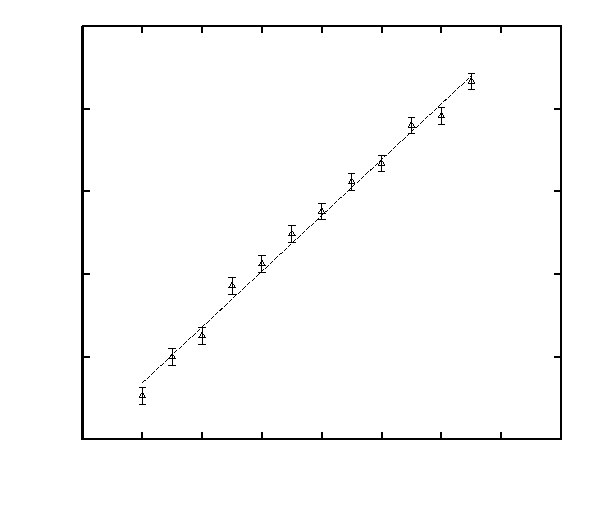
\includegraphics{least_squares}}%
    \gplfronttext
  \end{picture}%
\endgroup

\raisebox{4.55cm}{
\stdtablenocenter{3}
{$t$ (s) & $x$ (m) & $\Delta x$ (m)}
{$0.00$ & $1.57$ & $0.30$ \\
$0.10$ & $2.99$ & $0.30$ \\
$0.20$ & $3.75$ & $0.30$ \\
$0.30$ & $5.57$ & $0.30$ \\
$0.40$ & $6.36$ & $0.30$ \\
$0.50$ & $7.45$ & $0.30$ \\
$0.60$ & $8.27$ & $0.30$ \\
$0.70$ & $9.35$ & $0.30$ \\
$0.80$ & $10.01$ & $0.30$ \\
$0.90$ & $11.40$ & $0.30$ \\
$1.00$ & $11.74$ & $0.30$ \\
$1.10$ & $12.99$ & $0.30$ \\
}
}}
{Tabella dei dati relativi all'esempio \ref{esem:LeggeOrariaMinimiQuadrati}
e grafico relativo ai dati stessi. La retta di fit restituita da un fit
dei minimi quadrati \`e riportata sul grafico insieme ai punti
sperimentali.}
{fig:LeggeOrariaMinimiQuadrati}
I dati nella tabella sono stati simulati con un programma al calcolatore
assumendo che l'oggetto si muova lungo l'asse $x$ di moto rettilineo
uniforme:
$$
x(t) = x_0 + v_0 t
$$
con
\begin{eqnarray*}
x_0 & = & 2.3 \m\\
v_0 & = & 10 \m/{\rm s}
\end{eqnarray*}
ed ancora assumendo un errore di misura gaussiano sulle lunghezze con
deviazione standard pari a $0.3 \m$.
Le misure di tempo possono essere considerate abbastanza
accurate da far s\`i che la (\ref{eq:DeltaXTrascurabile}) sia verificata.

Notiamo esplicitamente che, avendo generato i dati al calcolatore, ci troviamo
nella posizione estremamente privilegiata di conoscere il valore dei
misurandi $x_0$ e $v_0$; cosa che, per ovvie ragioni, non \`e
di norma vera in laboratorio.
Questo ci permette di verificare in modo diretto la correttezza di un
dato algoritmo di analisi ed \`e un procedimento usato molto comunemente
nel progetto di esperimenti scientifici.

Applicando dunque i risultati appena derivati, un fit dei minimi quadrati
(abbiamo gi\`a verificato che le ipotesi necessarie siano verificate)
restituisce i seguenti valori:
\begin{eqnarray*}
x_0 & = & 2.05 \pm 0.16 \m\\
v_0 & = & 10.14 \pm 0.25 \m/{\rm s}\\
\end{eqnarray*}

che sono statisticamente compatibili (entro due $\sigma$) con i
valori dei misurandi, noti a priori.}

\end{exemplify}

\section{Metodo del minimo \texorpdfstring{$\chi^2$}{chi2}}

\index{minimo $\chi^2$!metodo di fit del}Supponiamo adesso che le incertezze
$\Delta y_i$ associate alle nostre misure siano, in generale, tutte diverse,
mentre manteniamo, per il momento, l'ipotesi che l'errore sulle $x_i$ sia
molto piccolo, nel senso della (\ref{eq:DeltaXTrascurabile}).
Il metodo dei minimi quadrati introdotto nel paragrafo precedente
pu\`o essere generalizzato a questa situazione introducendo
le quantit\`a:
$$
D_i = \frac{y_i - f(x; p_1 \ldots p_m)}{\Delta y_i}
$$
in cui ogni differenza viene {\itshape pesata} con l'inverso dell'errore
sulle misure $y_i$ (intuitivamente: maggiore \`e l'errore di misura,
minore \`e il peso che la misura stessa ha nel fit).
Si cercher\`a poi il minimo della funzione:
\eqnlbox{
S = \sum_{i=1}^n D_i^2 =
\sum_{i=1}^n\left[\frac{y_i - f(x; p_1 \ldots p_m)}{\Delta y_i}\right]^2
}{eq:SMinimoChiQuadro}
imponendo che le derivate rispetto a tutti i parametri siano nulle:
\eqn{
\left \{ \begin{array}{l}
\pfder{S}{p_1} = \pfder{}{p_1} \sum_{i=1}^n
\left[\frac{y_i - f(x; p_1 \ldots p_m)}{\Delta y_i}\right]^2 = 0\\
\pfder{S}{p_2} = \pfder{}{p_2} \sum_{i=1}^n
\left[\frac{y_i - f(x; p_1 \ldots p_m)}{\Delta y_i}\right]^2 = 0\\
\cdots \\
\pfder{S}{p_m} = \pfder{}{p_m} \sum_{i=1}^n
\left[\frac{y_i - f(x; p_1 \ldots p_m)}{\Delta y_i}\right]^2 = 0
\end{array} \right.
}

Questo metodo viene indicato come {\em il metodo del minimo $\chi^2$}.
Infatti se si assume che le $y_i$ abbiano una distribuzione gaussiana, le
$D_i$ sono variabili gaussiane con media zero e varianza uno ed $S$ \`e
una variabile che ha la distribuzione del $\chi^2$.


\subsection{Fit del minimo \texorpdfstring{$\chi^2$}{chi2} per una funzione
  costante: la media pesata}

\index{media pesata}
Supponiamo di eseguire un certo numero $n$ di misure {\itshape indipendenti}
di una stessa grandezza $y$ ottenendo $n$ valori $y_i$, in generali diversi
tra loro, con relative incertezze $\Delta y_i$, che pure ammettiamo poter
essere diverse tra di loro.
Ci poniamo il problema di valutare, a partire dai nostri dati,
la migliore stima per $y$ e l'incertezza associata.
Se potessimo trattare le misure tutte allo stesso modo (cio\`e se i
$\Delta y_i$
fossero tutti uguali), la migliore stima per $y$ sarebbe costituita dalla
media aritmetica delle $y_i$ (cfr. sezione \ref{subsec:FitMinQuadCostante}).
Ma se questa ipotesi cade \`e ragionevole aspettarsi, intuitivamente,
che le misure affette da incertezza maggiore debbano {\itshape contare}
meno delle altre.
Il problema si riduce, nel nostro linguaggio, ad un fit del minimo $\chi^2$
con una funzione costante:
$$
y = f(x; a)={\rm cost}=a
$$
Notiamo, per inciso, che la condizione (\ref{eq:DeltaXTrascurabile})
\`e qui automaticamente soddisfatta in quanto
$$
\tfdereval{f}{x}{x} = 0
$$
Costruiamo allora la somma:
$$
S = \sum_{i=1}^{n}\left(\frac{y_i-a}{\Delta y_i}\right)^2
$$
ed imponiamo che la derivata rispetto all'unico parametro sia nulla:
$$
\pfder{S}{a}=-2 \sum_{i=1}^{n} \frac{1}{\Delta y_i} \cdot
\left(\frac{y_i-a}{\Delta y_i}\right) = 0
$$
Questo fornisce:
$$
\sum_{i=1}^{n} \frac{y_i}{(\Delta y_i)^2} =
\sum_{i=1}^{n} \frac{a}{(\Delta y_i)^2} =
a \sum_{i=1}^{n} \frac{1}{(\Delta y_i)^2}
$$
ed infine:
\eqnlbox{
a = \frac{\displaystyle \sum_{i=1}^{n}
\frac{y_i}{(\Delta y_i)^2}}
{\displaystyle \sum_{i=1}^{n} \frac{1}{(\Delta y_i)^2}}
}{eq:MediaPesata}
L'incertezza associata si valuta come di consueto:
$$
(\Delta a)^2 = \sum_{i=1}^{n} \left(\pfder{a}{y_i}\right)^2 (\Delta y_i)^2 =
\frac{\displaystyle \sum_{i=1}^{n} \frac{1}{(\Delta y_i)^4}
\cdot (\Delta y_i)^2}
{\displaystyle \left[ \sum_{i=1}^{n} \frac{1}{(\Delta y_i)^2} \right]^2}=
\frac{\displaystyle \sum_{i=1}^{n} \frac{1}{(\Delta y_i)^2}}
{\displaystyle \left[ \sum_{i=1}^{n} \frac{1}{(\Delta y_i)^2} \right]^2}
$$
per cui:
\eqnlbox{
\Delta a = \frac{\displaystyle 1}
{\sqrt{\displaystyle \sum_{i=1}^{n} \frac{1}{(\Delta y_i)^2}}}}
{eq:ErroreMediaPesata}

\begin{exemplify}

\example{\label{esem:MediaPesata}
Si eseguono $5$ misure indipendenti dell'indice di rifrazione
dell'acqua ottenendo i risultati in tabella%
\footnote{
Dati realmente ottenuti negli anni accademici 2002-03, 2003-04, 2004-05.
}%
.
\stdtable{2}%
{$n_i$ & $\Delta n_i$}%
{$1.325$ & $0.012$\\
$1.3$ & $0.1$\\
$1.33$ & $0.01$\\
$1.331$ & $0.005$\\
$1.335$ & $0.006$\\}
Si vogliono combinare questi dati in modo da fornire una stima
statisticamente corretta di n. Assumendo che le incertezze riportate in
tabella siano state valutate correttamente e che gli effetti sistematici
siano stati tenuti sotto controllo, il modo corretto di procedere \`e quello
di eseguire una media pesata, secondo le equazioni (\ref{eq:MediaPesata}) e
(\ref{eq:ErroreMediaPesata}):
$$
n = 1.332 \pm 0.003
$$
Notiamo esplicitamente che la media aritmetica degli $n_i$ sarebbe
$1.324$, che \`e significativamente pi\`u bassa della media pesata
(sostanzialmente essa \`e influenzata dal valore della seconda misura che,
essendo affetta da un'incertezza relativa molto pi\`u grande degli altri,
conta meno nella media pesata).}

\end{exemplify}


\subsection{Fit del minimo \texorpdfstring{$\chi^2$}{chi2} nel caso lineare}
\label{sec:MinChiQuadroLineare}

In analogia alla sezione \ref{subsec:FitMinQuadLineare} applichiamo il
metodo del minimo $\chi^2$ al caso lineare:
$$
y = f(x; a, b) = a + b x
$$
Cominciamo dal costruire la somma:
$$
S = \sum_{i=1}^n\left(\frac{y_i - a - b x_i}{\Delta y_i}\right)^2
$$
e deriviamo rispetto ai parametri:
$$
\left \{ \begin{array}{l}
\pfder{S}{a} = -2\sum_{i=1}^{n} \frac{1}{\Delta y_i} \cdot
\left(\frac{y_i-a-b x_i}{\Delta y_i}\right) = 0\\
\pfder{S}{b} = -2\sum_{i=1}^{n} \frac{1}{\Delta y_i} \cdot
\left(\frac{y_i-a-b x_i}{\Delta y_i}\right)x_i = 0
\end{array} \right.
$$
da cui:
$$
\left \{ \begin{array}{l}
\displaystyle a \sum_{i=1}^{n} \frac{1}{(\Delta y_i)^2}
+ b \sum_{i=1}^{n} \frac{x_i}{(\Delta y_i)^2} =
\sum_{i=1}^{n} \frac{y_i}{(\Delta y_i)^2}\\
\displaystyle a \sum_{i=1}^{n} \frac{x_i}{(\Delta y_i)^2}
+ b \sum_{i=1}^{n} \frac{x_i^2}{(\Delta y_i)^2} =
\sum_{i=1}^{n} \frac{x_i y_i}{(\Delta y_i)^2}
\end{array} \right.
$$
Si ha infine:
\eqnbox{
\left \{ \begin{array}{l}
a=\frac{\displaystyle \sum_{i=1}^{n} \frac{y_i}{(\Delta y_i)^2}\cdot
\sum_{i=1}^{n} \frac{x_i^2}{(\Delta y_i)^2}
-\sum_{i=1}^{n} \frac{x_i}{(\Delta y_i)^2}\cdot
\sum_{i=1}^{n} \frac{x_i y_i}{(\Delta y_i)^2}}
{\displaystyle\sum_{i=1}^{n} \frac{1}{(\Delta y_i)^2}\cdot
\sum_{i=1}^{n} \frac{x_i^2}{(\Delta y_i)^2}-
\left(\sum_{i=1}^{n} \frac{x_i}{(\Delta y_i)^2}\right)^2} \\
\\
b=\frac{\displaystyle\sum_{i=1}^{n} \frac{1}{(\Delta y_i)^2}\cdot
\sum_{i=1}^{n} \frac{x_i y_i}{(\Delta y_i)^2}
-\sum_{i=1}^{n} \frac{y_i}{(\Delta y_i)^2}\cdot
\sum_{i=1}^{n} \frac{x_i}{(\Delta y_i)^2}}
{\displaystyle\sum_{i=1}^{n} \frac{1}{(\Delta y_i)^2}\cdot
\sum_{i=1}^{n} \frac{x_i^2}{(\Delta y_i)^2}-
\left(\sum_{i=1}^{n} \frac{x_i}{(\Delta y_i)^2}\right)^2}
\end{array} \right.}
ed ancora:
$$
\left \{ \begin{array}{l}
(\Delta a)^2=
\displaystyle\sum_{i=1}^{n}\left(\pfder{a}{y_i}\right)^2
\cdot (\Delta y_i)^2=
\frac{\displaystyle\sum_{i=1}^{n} \frac{x_i^2}{(\Delta y_i)^2}}
{\displaystyle\sum_{i=1}^{n} \frac{1}{(\Delta y_i)^2}\cdot
\sum_{i=1}^{n} \frac{x_i^2}{(\Delta y_i)^2}-
\left(\sum_{i=1}^{n} \frac{x_i}{(\Delta y_i)^2}\right)^2} \\
\\
(\Delta b)^2=
\displaystyle\sum_{i=1}^{n}\left(\pfder{b}{y_i}\right)^2
\cdot (\Delta y_i)^2=
\frac{\displaystyle\sum_{i=1}^{n} \frac{1}{(\Delta y_i)^2}}
{\displaystyle\sum_{i=1}^{n} \frac{1}{(\Delta y_i)^2}\cdot
\sum_{i=1}^{n} \frac{x_i^2}{(\Delta y_i)^2}-
\left(\sum_{i=1}^{n} \frac{x_i}{(\Delta y_i)^2}\right)^2}
\end{array} \right.
$$
da cui:
\eqnbox{
\left \{ \begin{array}{l}
\Delta a =
\frac{\sqrt{\displaystyle\sum_{i=1}^{n} \frac{x_i^2}{(\Delta y_i)^2}}}
{\sqrt{\displaystyle\sum_{i=1}^{n} \frac{1}{(\Delta y_i)^2}\cdot
\sum_{i=1}^{n} \frac{x_i^2}{(\Delta y_i)^2}-
\left(\sum_{i=1}^{n} \frac{x_i}{(\Delta y_i)^2}\right)^2}}\\
\\
\Delta b =
\frac{\sqrt{\displaystyle\sum_{i=1}^{n} \frac{1}{(\Delta y_i)^2}}}
{\sqrt{\displaystyle\sum_{i=1}^{n} \frac{1}{(\Delta y_i)^2}\cdot
\sum_{i=1}^{n} \frac{x_i^2}{(\Delta y_i)^2}-
\left(\sum_{i=1}^{n} \frac{x_i}{(\Delta y_i)^2}\right)^2}}
\end{array} \right.
}

\begin{exemplify}

\example{\label{esem:LeggeOrariaMinimoChiQuadro}I dati nella tabella
sono stati simulati con lo stesso programma dell'esempio
\ref{esem:LeggeOrariaMinimiQuadrati} con una piccola variante:
questa volta gli errori di misura sulle lunghezze non sono costanti
ma direttamente proporzionali alle lunghezze stesse, di modo che
l'errore relativo \`e costante e pari al $5\%$ (cfr. figura
\ref{fig:LeggeOrariaMinChiQuadro}).
\panelfig{
% GNUPLOT: LaTeX picture with Postscript
\begingroup
\footnotesize
  \makeatletter
  \providecommand\color[2][]{%
    \GenericError{(gnuplot) \space\space\space\@spaces}{%
      Package color not loaded in conjunction with
      terminal option `colourtext'%
    }{See the gnuplot documentation for explanation.%
    }{Either use 'blacktext' in gnuplot or load the package
      color.sty in LaTeX.}%
    \renewcommand\color[2][]{}%
  }%
  \providecommand\includegraphics[2][]{%
    \GenericError{(gnuplot) \space\space\space\@spaces}{%
      Package graphicx or graphics not loaded%
    }{See the gnuplot documentation for explanation.%
    }{The gnuplot epslatex terminal needs graphicx.sty or graphics.sty.}%
    \renewcommand\includegraphics[2][]{}%
  }%
  \providecommand\rotatebox[2]{#2}%
  \@ifundefined{ifGPcolor}{%
    \newif\ifGPcolor
    \GPcolorfalse
  }{}%
  \@ifundefined{ifGPblacktext}{%
    \newif\ifGPblacktext
    \GPblacktexttrue
  }{}%
  % define a \g@addto@macro without @ in the name:
  \let\gplgaddtomacro\g@addto@macro
  % define empty templates for all commands taking text:
  \gdef\gplbacktext{}%
  \gdef\gplfronttext{}%
  \makeatother
  \ifGPblacktext
    % no textcolor at all
    \def\colorrgb#1{}%
    \def\colorgray#1{}%
  \else
    % gray or color?
    \ifGPcolor
      \def\colorrgb#1{\color[rgb]{#1}}%
      \def\colorgray#1{\color[gray]{#1}}%
      \expandafter\def\csname LTw\endcsname{\color{white}}%
      \expandafter\def\csname LTb\endcsname{\color{black}}%
      \expandafter\def\csname LTa\endcsname{\color{black}}%
      \expandafter\def\csname LT0\endcsname{\color[rgb]{1,0,0}}%
      \expandafter\def\csname LT1\endcsname{\color[rgb]{0,1,0}}%
      \expandafter\def\csname LT2\endcsname{\color[rgb]{0,0,1}}%
      \expandafter\def\csname LT3\endcsname{\color[rgb]{1,0,1}}%
      \expandafter\def\csname LT4\endcsname{\color[rgb]{0,1,1}}%
      \expandafter\def\csname LT5\endcsname{\color[rgb]{1,1,0}}%
      \expandafter\def\csname LT6\endcsname{\color[rgb]{0,0,0}}%
      \expandafter\def\csname LT7\endcsname{\color[rgb]{1,0.3,0}}%
      \expandafter\def\csname LT8\endcsname{\color[rgb]{0.5,0.5,0.5}}%
    \else
      % gray
      \def\colorrgb#1{\color{black}}%
      \def\colorgray#1{\color[gray]{#1}}%
      \expandafter\def\csname LTw\endcsname{\color{white}}%
      \expandafter\def\csname LTb\endcsname{\color{black}}%
      \expandafter\def\csname LTa\endcsname{\color{black}}%
      \expandafter\def\csname LT0\endcsname{\color{black}}%
      \expandafter\def\csname LT1\endcsname{\color{black}}%
      \expandafter\def\csname LT2\endcsname{\color{black}}%
      \expandafter\def\csname LT3\endcsname{\color{black}}%
      \expandafter\def\csname LT4\endcsname{\color{black}}%
      \expandafter\def\csname LT5\endcsname{\color{black}}%
      \expandafter\def\csname LT6\endcsname{\color{black}}%
      \expandafter\def\csname LT7\endcsname{\color{black}}%
      \expandafter\def\csname LT8\endcsname{\color{black}}%
    \fi
  \fi
  \setlength{\unitlength}{0.0500bp}%
  \begin{picture}(5760.00,4888.80)%
    \gplgaddtomacro\gplbacktext{%
      \csname LTb\endcsname%
      \put(660,660){\makebox(0,0)[r]{\strut{} 0}}%
      \put(660,1453){\makebox(0,0)[r]{\strut{} 3}}%
      \put(660,2246){\makebox(0,0)[r]{\strut{} 6}}%
      \put(660,3039){\makebox(0,0)[r]{\strut{} 9}}%
      \put(660,3832){\makebox(0,0)[r]{\strut{} 12}}%
      \put(660,4625){\makebox(0,0)[r]{\strut{} 15}}%
      \put(792,440){\makebox(0,0){\strut{}-0.2}}%
      \put(1366,440){\makebox(0,0){\strut{} 0}}%
      \put(1940,440){\makebox(0,0){\strut{} 0.2}}%
      \put(2515,440){\makebox(0,0){\strut{} 0.4}}%
      \put(3089,440){\makebox(0,0){\strut{} 0.6}}%
      \put(3663,440){\makebox(0,0){\strut{} 0.8}}%
      \put(4237,440){\makebox(0,0){\strut{} 1}}%
      \put(4812,440){\makebox(0,0){\strut{} 1.2}}%
      \put(5386,440){\makebox(0,0){\strut{} 1.4}}%
      \put(220,2642){\rotatebox{90}{\makebox(0,0){\strut{}\gplabel{$x\;({\rm m})$}}}}%
      \put(3089,110){\makebox(0,0){\strut{}\gplabel{$t\;({\rm s})$}}}%
    }%
    \gplgaddtomacro\gplfronttext{%
    }%
    \gplbacktext
    \put(0,0){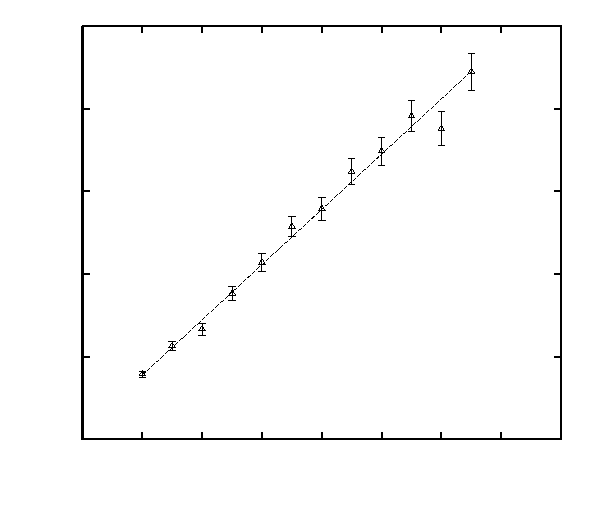
\includegraphics{least_chisquare}}%
    \gplfronttext
  \end{picture}%
\endgroup

\raisebox{4.55cm}{
\stdtablenocenter{3}
{$t$ (s) & $x$ (m) & $\Delta x$ (m)}
{$0.00$ & $2.36$ & $0.11$ \\
$0.10$ & $3.38$ & $0.17$ \\
$0.20$ & $4.00$ & $0.21$ \\
$0.30$ & $5.30$ & $0.27$ \\
$0.40$ & $6.42$ & $0.32$ \\
$0.50$ & $7.72$ & $0.36$ \\
$0.60$ & $8.37$ & $0.42$ \\
$0.70$ & $9.71$ & $0.47$ \\
$0.80$ & $10.46$ & $0.52$ \\
$0.90$ & $11.73$ & $0.57$ \\
$1.00$ & $11.27$ & $0.62$ \\
$1.10$ & $13.34$ & $0.67$ \\
}
}}
{Tabella dei dati relativi all'esempio \ref{esem:LeggeOrariaMinimoChiQuadro}
e grafico relativo ai dati stessi. La retta di fit restituita da un fit
del minimo $\chi^2$ \`e riportata sul grafico insieme ai punti sperimentali.}
{fig:LeggeOrariaMinChiQuadro}

Ammettendo di nuovo che gli errori sulle misure di tempo siano
trascurabili, secondo la (\ref{eq:DeltaXTrascurabile}), siamo nelle ipotesi
del minimo $\chi^2$. Il fit del minimo $\chi^2$ in effetti fornisce per
i parametri i seguenti valori:
\begin{eqnarray*}
x_0 & = & 2.33 \pm 0.09 \\
v_0 & = & 10.03 \pm 0.28 \\
\end{eqnarray*}

che di nuovo sono compatibili con i misurandi.

Se avessimo applicato il metodo dei minimi quadrati---procedimento
statisticamente non corretto, in questo caso, dato che gli errori di misura
sono diversi tra loro---avremmo ottenuto:
\begin{eqnarray*}
x_0 & = & 2.41 \pm 0.06 \m\\
v_0 & = & 9.87 \pm 0.10 \m/{\rm s}\\
\end{eqnarray*}

In questo caso le stime dei parametri sono leggermente peggiori (come \`e
logico aspettarsi), sia pure ancora ragionevoli; gli errori sui parametri
stessi, viceversa, sono un artefatto del fit e non devono essere presi
seriamente.}

\end{exemplify}


\section{Fit di tipo generale}
Nei metodi finora discussi abbiamo sempre supposto che l'errore sulle $x_i$
fosse trascurabile, e come tale l'abbiamo trattato. Finora ci siamo quindi
occupati di casi relativamente semplici. Relativamente, s'intende, al caso
che esamineremo adesso: vogliamo infatti studiare il problema di fitting nel
caso pi\`u generale in cui non sono trascurabili n\'e gli errori su $y$ n\'e
quelli su $x$.

Il primo problema che si incontra \`e che in un'equazione del tipo
$y = f(x; p_1 \ldots p_m)$ non \`e chiaro quale sia il valore da usare per
$x$ in modo da calcolare il valore teorico di $y$ e quindi cercare i migliori
valori dei parametri che soddisfino la richiesta di rendere minimo il $\chi^2$.
Non conoscendo $x$ il problema \`e quindi concettualmente pi\`u
complicato: bisogna determinare i valori di $(\tilde{x_i}, \tilde{y_i})$
tali che sia minimo
\eqn{
\sum_{i=1}^n\left[\left(\frac{\tilde{x_i}-x_i}{\Delta x_i}\right)^2 +
\left(\frac{\tilde{y_i}-y_i}{\Delta y_i}\right)^2\right]
}
con la condizione che
\eqn{
{\cal F}(\tilde{x_i}, \tilde{y_i}; \, p_1 \ldots p_m)=0
\qquad\forall i= 1\ldots n
}
dove ${\cal F}(x, y; \, p_1 \ldots p_m)$  \`e la relazione che si
vuole che leghi la $x$ alla $y$ scritta in forma implicita.

Si tratta di un problema di minimo condizionato: usando il metodo dei
{\itshape moltiplicatori di Lagrange} ci si riduce al problema seguente:
minimizzare
\eqnl{
S = \sum_{i=1}^n\left[\left(\frac{\tilde{x_i}-x_i}{\Delta x_i}\right)^2+
\left(\frac{\tilde{y_i}-y_i}{\Delta y_i}\right)^2+
\lambda_i {\cal F}(\tilde{x_i}, \tilde{y_i}; \, p_1 \ldots p_m)\right]
}{eq:SGenerale}
Le cose da determinare sono $\tilde{x_i}$, $\tilde{y_i}$, $\lambda_i$,
$p_1 \ldots p_m$: in tutto $3n+m$;
ci sono quindi derivate parziali rispetto a $3n+m$ variabili.

Il problema si pu\`o risolvere nel caso pi\`u generale solo con metodi
numerici approssimati.
Diamo alcuni cenni sulla tecnica di risoluzione:
\begin{numlist}
\item{
Il primo passo \`e di conoscere un valore approssimato dei parametri.
}
\item{
Il secondo passo \`e di usare invece di  ${\cal F}(x, y; \, p_1 \ldots p_m)$
la sua approssimazione al prim'ordine. Pertanto ad 
${\cal F}(x, y; \, p_1 \ldots p_m)$ viene sostituita una funzione lineare.
}
\item{
Quindi c'\`e una certa quantit\`a di algebra, sostituzioni, ecc.
}
\item{
Il risultato \`e un sistema di equazioni lineari che dicono di quanto
devono essere corrette le stime iniziali dei parametri.
}
\item{
A questo punto si procede con metodo iterativo, cio\`e si prendono i
nuovi valori dei parametri e si ricomincia.
}
\item{
Se il processo converge alla fine si ottengono i valori richiesti
per i parametri.
}
\end{numlist}

\begin{exemplify}

\example{Analizziamo in dettaglio la procedura generale di fit nel caso
puramente lineare%
\footnote{Per le funzioni che, come questa, sono lineari nei parametri,
potrebbero essere usati metodi pi\`u semplici (provate).
Tuttavia la semplicit\`a dell'esempio permette di seguire
meglio la tecnica proposta.}%
:
$$
y = f(x; \, p) = p x
$$
La forma implicita della funzione che lega la $y$ alla $x$ si scrive come:
$$
{\cal F}(x, y; \, p) = y - p x = 0
$$
Costruiamo allora la somma (\ref{eq:SGenerale}):
$$
S = \sum_{i=1}^n\left[\left(\frac{\tilde{x_i} - x_i}{\Delta x_i}\right)^2+
\left(\frac{\tilde{y_i} - y_i}{\Delta y_i}\right)^2 +
\lambda_i(\tilde{y_i} - p\tilde{x_i})\right]
$$
Le condizioni di minimo sono:
$$
\left\{\begin{array}{l}
\pfder{S}{\tilde{x_i}}=\frac{2(\tilde{x_i}-x_i)}{(\Delta x_i)^2}-\lambda_i p=0
\vspace{0.2cm}\\
\pfder{S}{\tilde{y_i}}=\frac{2(\tilde{y_i}-y_i)}{(\Delta y_i)^2}-\lambda_i=0
\vspace{0.2cm}\\
\pfder{S}{\lambda_i}=\tilde{y_i} - p\tilde{x_i} = 0
\vspace{0.2cm}\\
\pfder{S}{p} = - \dsum{\lambda_i \tilde{x_i}}{i}{1}{n} \approx
- \dsum{\lambda_i x_i}{i}{1}{n} = 0
\end{array}\right.
$$
Dove nell'ultima relazione si \`e linearizzata la $\cal F$.
Si ricavano $\tilde{x_i}$ ed $\tilde{y_i}$ dalle prime due relazioni:
$$
\left\{\begin{array}{l}
\displaystyle \tilde{x_i} = \frac{\lambda_i p \cdot (\Delta x_i)^2}{2} + x_i
\vspace{0.2cm}\\
\displaystyle \tilde{y_i} = \frac{\lambda_i \cdot (\Delta y_i)^2}{2} + y_i
\end{array}\right.
$$
e si sostituiscono nella terza:
$$
\frac{\lambda_i \cdot (\Delta y_i)^2}{2} + y_i -
\frac{\lambda_i p^2 \cdot (\Delta x_i)^2}{2} - x_i = 0
$$
da cui si ricava $\lambda_i$:
$$
\lambda_i = \frac{2(y_i - p x_i)}{p^2 \cdot (\Delta x_i)^2 + (\Delta y_i)^2}
$$
che, sostituito nella quarta relazione d\`a:
\eqnl{
p'=\frac{\displaystyle
\dsum{\frac{x_i y_i}{p^2 \cdot (\Delta x_i)^2 + (\Delta y_i)^2}}{i}{1}{n}}
{\displaystyle
\dsum{\frac{x_i^2}{p^2 \cdot (\Delta x_i)^2 + (\Delta y_i)^2}}{i}{1}{n}}
}{eq:FitGeneraleRetta}
a questo punto entra in funzione il metodo iterativo: si stima $p$ (ad esempio
dal grafico) e si usa questa stima nel secondo membro della
(\ref{eq:FitGeneraleRetta}) ottenendo un nuovo $p$ (chiamato $p'$), si ripete
il procedimento fino a quando la differenza fra i successivi valori di $p$ \`e
entro l'errore su $p$.

Per stimare gli errori su $p$ si usano l'equazione (\ref{eq:FitGeneraleRetta})
e le tecniche della propagazione degli errori ed il valore stimato di $p$:
$$
(\Delta p)^2=
\dsum{\left[\left(\pfder{p}{x} \cdot \Delta x_i \right)^2+
\left(\pfder{p}{y} \cdot \Delta y_i \right)^2 \right]}{i}{1}{n}
 =\frac{1}{\displaystyle\sum_{i=1}^{n}\frac{x_i^2}{p^2\cdot(\Delta x_i)^2 +
(\Delta y_i)^2}}
$$}

\end{exemplify}


\section{Test del \texorpdfstring{$\chi^2$}{chi2}}
\label{sec:TestChiQuadro}


\index{$\chi^2$!test del}Richiamiamo la definizione della variabile $\chi^2$ a
$n$ gradi di libert\`a: date $n$ variabili $x_i$ gaussiane con media $\mu_i$ e
deviazione standard $\sigma_i$ e costruite le variabili standard
$$
z_i=\frac{x_i-\mu_i}{\sigma_i}
$$
la quantit\`a
\eqn{
S=\sum_{i=1}^n z_i^2 = \sum_{i=1}^n\left(\frac{x_i-\mu_i}{\sigma_i}\right)^2
}
\`e distribuita secondo la funzione di distribuzione del $\chi^2$
ad $n$ gradi di libert\`a, che \`e data dalla (\ref{eq:ChiQuadro}).
La media e la varianza valgono rispettivamente:
\begin{eqnarray*}
\mu_S &=&n\\
\sigma_S^2&=&2n
\end{eqnarray*}

Fissato il numero di gradi di libert\`a $n$, le tavole riportate nelle
appendici \ref{app:ChiQuadro1} e \ref{app:ChiQuadro2} forniscono
il valore $\gamma$ per cui la probabilit\`a che $S$ sia
minore di $\gamma$ sia uguale ad un certo valore $\wp$:
$$
\prob{S\le\gamma} = \wp
$$

\begin{exemplify}

\example{Sia $n=10$; ci si domanda quale sia il valore $\gamma$ tale che:
$$
\prob{S \le \gamma} = 95\%
$$
Il risultato si legge direttamente nella tavola in appendice
\ref{app:ChiQuadro1} ed \`e:
$$
\gamma = 18.308
$$}

\end{exemplify}


\subsection{Test del \texorpdfstring{$\chi^2$}{chi2} per una serie di misure}

Il $\chi^2$ pu\`o fornire un criterio generale ed obiettivo per decidere
se una certa equazione o una certa legge descriva bene oppure no i risultati
sperimentali.
Supponiamo, al solito, di aver misurato le quantit\`a $(x_i, y_i)$ legate
tra di loro da una funzione $y = f(x; p_1 \ldots p_m)$, la cui forma viene
ipotizzata in base a considerazioni fisiche, ed i cui parametri
$p_1 \ldots p_m$ sono determinati con uno dei metodi di fit discussi prima,
per esempio il metodo dei minimi quadrati o del minimo $\chi^2$.
Il $\chi^2$ in questo caso vale
$$
S=\sum_{i=1}^n \left[
\frac{y_i - f(x_i; p_1 \ldots p_m)}{\Delta y_i} \right]^2
$$
La quantit\`a $S$ viene spesso indicata con il nome di \emph{somma dei
residui}; intuitivamente \`e chiaro che, quanto pi\`u $S$ \`e grande, tanto
pi\`u la curva teorica si discosta dai punti sperimentali.

Supposto che gli errori siano stati valutati in modo corretto, andiamo a vedere
qual \`e il significato da attribuire al numero $S$.
Si cerca sulle tavole in corrispondenza al numero di gradi di libert\`a
dove si trova il valore $S$. Quando si fa un fit il numero di gradi di
libert\`a $\nu$ \`e il numero $n$ delle misure meno il numero $m$ di parametri
della funzione $f(x; p_1 \ldots p_m)$
\eqnl{
\nu=n-m
}{eq:nGradiDiLiberta}

\begin{exemplify}

\example{Supponiamo di aver ottenuto $S=7.2$ con $\nu=5$.
Dalla tavola in appendice \ref{app:ChiQuadro1} si ottiene:
$$
\prob{\chi^2\le S} \approx 80\%
$$
Questo significa che ripetendo le misure tante volte
ci si aspetta che nell'$80\%$ dei casi si otterr\`a un valore minore
di $7.2$; cio\`e $7.2$ \`e un valore non molto buono per il $\chi^2$,
ma nemmeno assurdo, nel $20\%$ dei casi pu\`o succedere che venga un risultato
pi\`u alto.

Per inciso: $\prob{\chi^2\ge S}$ viene solitamente chiamato livello di
significativit\`a ed \`e ovviamente:
$$
\prob{\chi^2\ge S} = 1 - \prob{\chi^2\le S}
$$}

\example{Nel caso dell'esempio \ref{esem:LeggeOrariaMinimiQuadrati} il
valore di $S$ restituito dal fit vale:
$$
S = 12.47 \qquad (\nu = 10)
$$

Il livello di significativit\`a del fit \`e dunque circa il $75 \%$, come
si legge in appendice \ref{app:ChiQuadro1}.}

\example{Nel caso dell'esempio \ref{esem:LeggeOrariaMinimoChiQuadro}
il valore di $S$ restituito dal fit del minimo $\chi^2$ vale:
$$
S = 8.00 \qquad (\nu = 10)
$$

mentre quello restituito dal fit dei minimi quadrati:
$$
S = 8.76 \qquad (\nu = 10)
$$

Il lettore non dovrebbe essere stupito dal fatto che $S$ sia
pi\`u piccolo nel caso del fit del minimo $\chi^2$ (i nomi non sono
in genere scelti a caso).}

\end{exemplify}

Convenzionalmente si accetta come limite $\prob{\chi^2\le S}$ per i risultati
buoni quello del $95\%$ da un lato, e quello del $5\%$ dall'altro, perch\'e,
anche se a prima vista sembra che la cosa migliore sia ottenere dei $\chi^2$
molto piccoli (o addirittura zero), in realt\`a questi casi vanno guardati con
sospetto. Di solito $\chi^2$ piccoli si ottengono perch\'e gli errori
sono sovrastimati, oppure i risultati sono truccati,
cio\`e lo sperimentatore (consciamente o no) tende ad attribuire al
risultato delle misure il valore che gli piacerebbe.
Esistono tuttavia altri livelli di significativit\`a a seconda dei
particolari problemi studiati. \`E comunque buona regola indicare sempre
quale \`e il valore del $\chi^2$ ottenuto e quindi la probabilit\`a del
$\chi^2$ associata alle ipotesi fatte ed ai parametri dedotti dalle misure.


\subsection{Test del \texorpdfstring{$\chi^2$}{chi2} per una distribuzione}

Supponiamo di fare un esperimento che abbia come oggetto l'osservazione
di $n$ possibili eventi $E_1 \ldots E_n$ e registriamo le
occorrenze $o_1 \ldots o_n$ di ciascuno di questi possibili eventi%
\footnote{
Le occorrenze osservate vengono generalmente indicate con la lettera $o$
dall'inglese \emph{observed}, che significa appunto \emph{osservato}.
}%
.
D'altra parte possiamo fare certe ipotesi
sul fenomeno che stiamo studiando le quali ci permettono di determinare
le occorrenze teoriche%
\footnote{
Le occorrenze teoriche si indicano solitamente con la lettera $e$ dall'inglese
\emph{expected} che significa \emph{atteso}.
}
$e_1 \ldots e_n$. Ci saranno
differenze tra le occorrenze osservate e quelle teoriche. Per determinare
se le differenze sono significative (e quindi eventualmente rifiutare
le ipotesi che hanno portato a calcolare gli $e_i$) si usa la quantit\`a
\eqnl{
S = \sum_{i=1}^n\frac{(o_i-e_i)^2}{e_i}
}{eq:ChiQuadroDistribuzione}
che viene considerata ancora una variabile $\chi^2$.
Formalmente ricorda un $\chi^2$ perch\'e si suppone che sia Poissoniana la
distribuzione di ognuna delle occorrenze $o_i$: $e_i$ rappresenta il valor
medio della parent distribution  e per una variabile Poissoniana la varianza
coincide con la media, per cui $\sigma^2_{o_i} = e_i$.
\`E tuttavia importante ricordare che  $o_i$ ed $e_i$ non sono variabili
gaussiane; o meglio: lo sono soltanto in condizioni limite,
cio\`e per $o_i$ (e quindi $e_i$) grande. In queste condizioni la
(\ref{eq:ChiQuadroDistribuzione}) tende ad una variabile $\chi^2$; $o_i>3$
\`e una condizione sufficiente per la maggior parte dei casi
che si incontrano in pratica.

I {\itshape \em gradi di libert\`a} sono $n-m-1$ dove $n$ \`e il numero delle
classi (cio\`e il numero degli eventi possibili) ed $m$ \`e il numero dei
parametri che servono per calcolare le occorrenze teoriche
$e_1 \ldots e_n$; inoltre deve essere soddisfatta la seguente relazione:
$$
\sum_{i=1}^n o_i=N
$$
dove $N$ \`e il numero totale delle osservazioni,
e questa relazione causa la perdita di un ulteriore grado di libert\`a.
Nel limite in cui la quantit\`a (\ref{eq:ChiQuadroDistribuzione})
pu\`o essere considerata un $\chi^2$ ad essa si
attribuisce lo stesso significato probabilistico trattato precedentemente.

\begin{exemplify}

\example{Si supponga di avere un foglio di carta diviso in 64 quadrati
numerati (da $1$ a $64$).
Si prendono 64 dischi e si lasciano cadere sul foglio di carta
uno alla volta, in modo che si distribuiscano pressoch\'e uniformemente
sul quadrato. Quindi si fa una tavola suddividendo i quadrati in funzione
del numero dei dischi che essi contengono:
\stdtable{3}%
{$k$ & $o_k$ & $e_k$}%
{$0$ & $21$ & $23.54$\\
$1$ & $26$ & $23.54$\\
$2$ & $13$ & $11.77$\\
$3$ & $4$ & $3.22$\\
$4$ & $0$ & $0.38$\\}
Per calcolare le frequenze teoriche, si \`e fatta l'ipotesi che
la distribuzione della variabile $k$ sia una Poissoniana con media
$1$ ($64$ dischi in $64$ quadrati cio\`e in media un disco
per quadrato):
$$
\prob{k}=\frac{1^k}{k!}e^{-1}=\frac{1}{k!}\cdot \frac{1}{e}
$$
Le frequenze teoriche si calcolano moltiplicando $\prob{k}$ per il numero
totale $n=64$ dei quadrati:
$$
e_k=\frac{1}{k!} \cdot \frac{64}{e}
$$
Calcoliamo il valore $S$ del $\chi^2$:
\begin{eqnarray*}
S &=& \sum_{i=0}^3\frac{(o_i-e_i)^2}{e_i}=\\
&=& \frac{(21-23.54)^2}{23.54}+ \frac{(26-23.54)^2}{23.54}+
\frac{(13-11.77)^2}{11.77}+\frac{(4-5.15)^2}{5.15} \approx 0.91
\end{eqnarray*}
I gradi di libert\`a sono $4-0-1=3$ (qui nessun parametro \`e
stato ricavato dalle misure: questa \`e una Poissoniana limite di una
Binomiale in cui sia $n$ che $p$ sono noti). Utilizzando le tavole
si trova:
$$\prob{\chi^2\le S} \approx 22\%.$$\normalsize}

\example{\label{esem:Lotto}L'istogramma in figura \ref{fig:LottoBA}
si riferisce ai numeri del gioco del lotto usciti nella ruota di Bari dal
1937 ad oggi. Per ognuna delle possibili uscite $k$ ($k = 1 \ldots 90$) \`e
riportato il numero di volte in cui essa si \`e verificata.
\panelfig
{\onebyonetexfig{./pp_fit/figure/lotto_BA.tex}}
{Istogramma in frequenza delle uscite del gioco del lotto sulla ruota di Bari
dal $1937$ ad oggi.}
{fig:LottoBA}

I dati si riferiscono a 4223 estrazioni; ricordiamo che ogni volta vengono
estratti 5 numeri (senza rimpiazzo) per cui ogni numero ha una probabilit\`a
di essere estratto pari a $\frac{5}{90}$.
Se il gioco non \`e truccato ci aspettiamo che il numero medio $e_k$ di uscite
per il numero $k$ in 4223 estrazioni sia uguale per tutti e pari a:
$$
e_k = 4223 \cdot \frac{5}{90} \approx 234.6 \qquad k = 1\ldots 90
$$
Un test del $\chi^2$ su questa distribuzione restituisce una somma dei
residui pari a:
$$
S = 98.313
$$
Il numero di gradi di libert\`a \`e qui $\nu = 90 - 0 - 1$ per cui il
livello di significativit\`a \`e pari a circa il $75\%$.
Con i dati in nostro possesso dobbiamo accettare l'ipotesi che il gioco non
sia truccato (per lo meno nel senso del $\chi^2$).}


\end{exemplify}


